\section{Svingsensor}
\label{svingsensor}
For at bilen kan detekterer og gemme at der er et sving, skal den udstyres med en sensor der kan kende forskel på lige strækninger og sving. Det vides at bilen bliver påvirket af en centripetalkraft, når den kører inde i et sving. For at kunne måle denne kraft, bruges der et accelerometer. Der var to accelerometer til rådighed; et digitalt (LIS35DE) og et analogt (MMA1270KEG). Først blev det digitale valgt, da dette har interrupt pins, som kunne være brugt til intelligent banedetektion. Grundet problemer med kommunikation mellem det digitale accelerometer og microcontrolleren, faldt valget på det analoge accelerometer.

\begin{figure}[h!]
\center
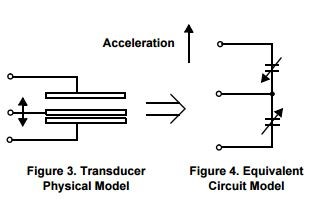
\includegraphics[scale=1]{./Graphics/Acceleration}
\caption{Accelerometer opbygning}
\label{Acceleration}
\end{figure}

\subsection{Hardware - MMA1270KEG}
Det analoge accelerometer er opbygget som vist på figur \ref{Acceleration}. Det kan ses som tre plader, hvor de to yderste er fikseret og den midterste kan bevæge sig. Den midterste plade bevæger sig derved med kraften og kapaciteten ændres mellem den midterste og de to fikserede plade. Den samlede kapacitans er konstant. Dette kan beskrives ved $(C=\frac{A\epsilon}{D})$, hvor A er arealet af pladerne, $\epsilon$ er den diaelektriske konstant og D er afstanden mellem den midterste plade og en af de to fikserede plader. Denne kapacitet bliver behandlet inde i accelerometeret af et kredsløb\footnote{Se side 4 af datablad for MMA1270KEG i bilag \ref{MMA1270KEG}}. Dette kredsløb sørger for at output signalet på accelerometeret er proportionalt med kraften.

\begin{figure}[h!]
\centering
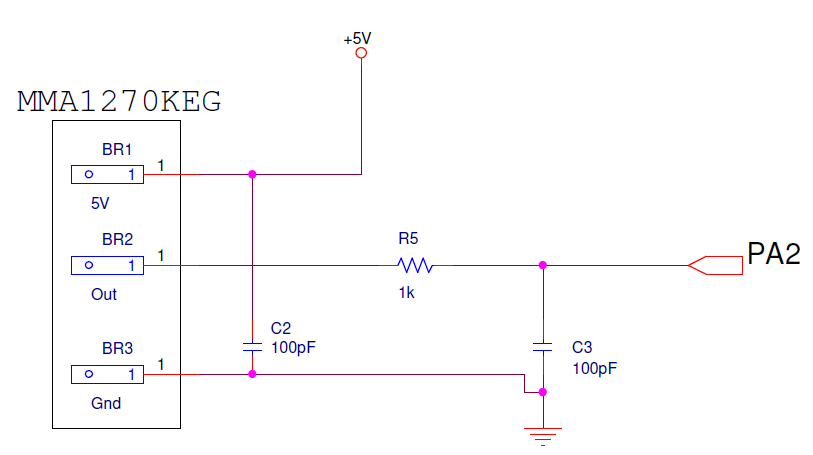
\includegraphics[scale=0.6]{./Graphics/Accelerometer_diagram}
\caption{Kredsløbs diagram over accelerometer}
\label{diagram_acc}
\end{figure}

Ved 0G er outputtet typisk på 2,5V og en sensitivitet på $750\frac{mV}{G}$.\footnote{Se Tabel 2, side 3 i databladet for MMA1270KEG i bilag \ref{MMA1270KEG}} \\
Output signalet er et signal der ligge mellem 0-5V og kan læses med en ADC af microcontrolleren.
Der er lavet er Lowpassfilter på output signalet fra accelerometeret, for at sortere de høje frekvenser fra. Der blev konstrueret det samme Lowpassfilter som blev forslået i databladet for sensoren. Altså en modstand på 1K\ohm og en capacitor på 100 nF. Dette giver en cut-off frekvens på:\\$f_{c}=\frac{1}{2\pi\tau}=\frac{1}{2\pi*RC}=1591.5 Hz$\\
Dette Lowpassfilter blev dog ikke optimeret grundet tidsmangel og der tages derfor højde for dette i koden.\\

\subsection{Software}
Til at læse sensoren, anvendes en analog indgang på microcontrolleren. ADC'en opsættes med en prescale på 128, da ADC'en max kan køre med 200 kHz og microcontrolleren kører med 16 MHz. \\
Når accelerometeret skal læses kaldes en subrutine. Denne subrutine sætter referencespændningen til 5V og vælger at "PA2" skal læses ind i ADC'en. Derefter venter programmet på at ADC'en er klar til at blive læst. Nå den er klar, læses værdien af ADC'en over i et register, som nu kan bruges til databehandling i programmet.\\

\begin{figure}[h!]
\centering
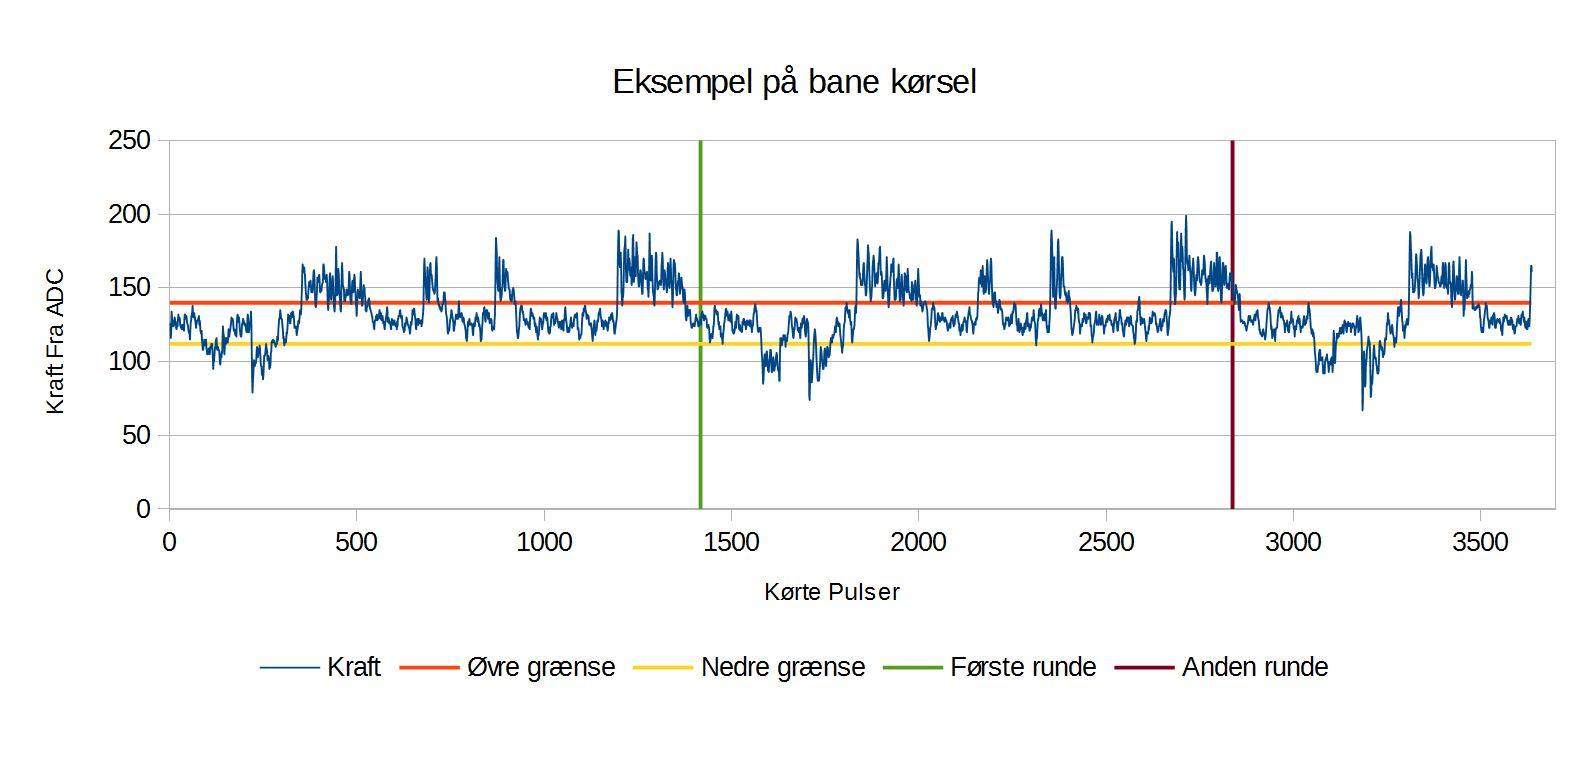
\includegraphics[scale=0.25]{./Graphics/banekorsel}
\caption{Graf over accelerometerdata fra testbanen. Testbane kan ses i bilag \ref{testbanebillede}}
\label{testbanegraf}
\end{figure}

Det ses at svingende er til at detektere, og farten aftager rundt i svingene. Dette diskuteres i afsnit \ref{sving}. På figur \ref{testbanegraf} ses et sving hvor den øvre grænse er indtegnet.\\

I figur \ref{testbanegraf} ses det at når bilen kører lige ud, er accelerometerværdien mellem den øvre grænsen (rød) og den nedre grænse (gul). I nogle tilfælde vil der grundet støj fås fejlmåling. Dette bliver der taget højde for ved at der skal være et antal på hinanden følgende målinger, som ligger under den øvre grænse, før det konstateres at bilen er ude af svinget. Denne metode bruges også i starten af et sving, da dette vil eliminere muligheden for at bilen tror den er i et sving, hvis der blot er tale om støj ved ligeud kørsel.\\



